Shelby Solomon's individual development plan is based on the strengths and weaknesses listed in section~\ref{sec:weaknesses} and will build off of the background~\ref{sec:background}.

\subsection{Technical \& Research Aims}
\begin{description}
	\item[Aim 1] Create a specialized google-type gene-rank mechanism by ranking genes found in GWAS/QTL mapping using public data sources. 
	\item[Rationale] The point of gene-rank mechanism, at least the version most suitable to our aims, is to give researchers interesting sets of genes to study given a specific focus area.
For instance, when attempting to understand addiction the ability to both search over as many accessible sources as possible finding genes related to the topic and then being able to rank the `goodness' of the genes in a way that fits your `goodness' definition is a much desired tool for omics researchers.
Gunturkun\cite{Gunturkun:2022} et. al. have done the first part of this work at UTHSC with Pjotr Prins. 
They have developed \textit{Genecup}, a tool that mines for gene-keyword relationships from PubMed and the genome wide association studies catalogue\cite{Buniello:2019}.
Machine learning is used to disambiguate search topics, while the tool searches abstracts and finds genes with keywords together in the same sentence.
The tool builds an ontology to help support the searching of the databases, and upon fetching the information develops an interactive graph using the keywords, genes and articles it finds.
As the graph is interactive one can select nodes and investigate sentences from the abstracts that result from the user query.

Moving beyond this utility a gene-ranking mechnanism will be applied to the resultant genes listed with the returned results.
Why gene-ranking, because it can highlight genes and haplotypes -- a physical grouping of genomic variants that tend to be inherited together that typically reflects a unique combination of variants that reside near each other on a chromsome that can include a single or multiple genes \cite{NHGRI:Haplotype}.
We will quickly elaborate on some of the techniques before describing our methods.
	\item[Methods] One of the \GN\ innovative outcomes is to build a more powerful database system combining human and model organisms, where Mouse and rat will be combined in one data resource.
Data entry methods will undergo improvement by way of controlled vocabularies and ontologies to cover genotypes and phenotypes.
The improved database will use RDF+SPARQL which are technologies designed to make information on the web more interconnected and accessible.
Another added beauty of these technologies is that they are designed to speed up data access and querying, and most especially work optimally with AI tools.
Such linked data is explicitly encoded in a standardized machine-readable syntax with relations useful for machine learning exercises\cite{toh2019}.
Gene rank learner is a tool that will rely on data from multiple sources: pubmed, wikidata, \GN\, rat genome database (\href{http://rgd.mcw.edu}{RGD}), the gene expression omnibus (GEO)~\cite{NCBIGeo}, the search tool for the retrieval of interacting genes (STRING~\cite{STRING}), the database for annotation visualization and integrated discovery (DAVID~\cite{DAVID}), a new human gene database collected from volunteers~\cite{henderson2020}, and more.
One of the major aspects of this software will be a data management service that pulls ontologies, schema and other functional data information so that querying data from different sources is done transparently as if there is one large data source. 
In essence, creating a sort of data lake with bridges to different sources and an adaptive interface that supports quick addition of more data sources.
The initial algorithm implemented will be gene rank product used by Zeng et.al. in \cite{zeng2016discovering}, along with a function to count fold changes.
Correlation and consistency algorithms will be implemented next, as they take gene expression information into account, improving upon the significance of micro arrays (SAM) methods that would focus on gene expression yet were outperformed by gene rank product in the past.
An ant colony optimizer (ACO)~\cite{ACO:2009} will be implemented to traverse the large graph that will be created from the accumulation of data from the various sources.
ACO looks for optimal solutions using graph traversal; hence, we must define what we think to be a possible optimal set of interesting genes based off of a genes many characteristics.
Each of these algorithms will be compared against one another by being made available to the \GN\ community.
Those who use the gene rank learner will be encouraged to provide feedback.
Before being released to the \GN\ community we will provide multiple definitions of interesting genes, and compare the efficacy of the results from each technique.
This ensemble of algorithms will be implemented in the Julia programming language, some of the packages that will be used are \hyperlink{https://www.juliapackages.com/p/antcolony}{a package for using ant colony optimization -- antcolony}, \hyperlink{https://juliapackages.com/p/evolutionary}{a package for evolutionary computations -- evolutionary}, \hyperlink{https://juliapackages.com/p/mxnet}{a package to run ML algorithms with GPU optimization -- MXNet}, and the \hyperlink{https://alan-turing-institute.github.io/MLJ.jl/dev/}{a general ML framework -- MLJ}.
\end{description}

\begin{description}
	\item[Aim 2] Take human data collected by the BIG project and place it into a GeneNetwork clone database that is not fully open to the public due to the nature of human data ownership.
	\item[Concept] \GN\ is a systems genetic database whose development is funded by the NIH. As such it follows FAIR principles, uses open source software (OSS), and provides tools for researchers and citizen scientists alike. As \GN\ continues to progress it will be a flagship genetic database for the NIH given the effort and expertise brought to the fore concerning its development.
	\item[Idea] Shelby Solomon will use the most current source base for \GN\ which uses RDF+SPARQL for faster querying while connecting to multiple online sources. Upon setting up an empty version of \GN\ with the most up-to-date tools and code, including the Generank algorithm, the DNA sequences of the thousands of volunteers who have agreed to be part of the BIG project will be input. The system will then be hardened against unauthorized and authorized usage using secure logins, cryptography and possibly biometrics authentication.
\end{description}

\begin{description}
	\item[Aim 3] Begin an investigation into causality for understanding why diabetes affects blacks in a disproportionate manner, and how the situation can be improved.
	\item[Concept] Diabetes is unfortunately a prevalent illness that has an oversized effect on underrepresented American populations; including Natives, Blacks, and Mexican \cite{Winer:2004}. Diabetes can lead to renal (kidney) failure among many other live imperiling issues.
	\item[Idea] Based on a quick analysis of diabetes and its causes a causal diagram is presented in ~\ref{fig:diabetes-cm}. In thinking through a causal diagram for diabetes, because its complications lead to so many other serious issues in underrepresented communities, we need to look at causes that mediate and ones that are confounders.
 A list of causes that can be evaluated: damage to the pancreas, obesity, specific medicines, high cholesterol, age, family history and certain hormonal conditions/imbalances. 
 The following list are things that are not easily evaluated or known: genetic predisposition, genetic mutation, lifestyle, gestational complications, and chance.
In the causal diagram `genetic mutation', healthcare access, and lifestyle all connect to the outcome diabetes through mediators.
Mediators are like symptoms to a problem, while explaining a known subset of a cause a mediator does not encompass the full probability of a cause that effects a specific outcome.
Even with mediators the furthest causes from the outcome do not all have a direct line to the outcome in our diagram in order to make the diagram less confusing and complicated.
A much more simple diagram could have been created with three nodes with the two cause nodes representing the group of observable causes and the group of un-observable causes both having a direct connection to the diabetes outcome.
However, this oversimplification does not help with showing the minimal complexity for the onset of diabetes.
For instance, `genetic mutation' is un-observable, as is `genetic predisposition' while both being confounders.
Also when looking at the several mediators from `genetic mutation' I am using `genetic predisposition' as a catch all past the mutation, since there are three other mediators based off of that single cause.
These causes are Confounders because especially as combined with `family history' and `lifestyle' can be interchanged and swapped and reach the diabetes outcome, with high probability while also being able to `prevent' diabetes if any one is not attributable to an individual.
Then there are causes like `age' and `specific medicines' that can directly bring the onset of diabetes while not logically being able to be a lone catalyst for the same.
However, the diagram must be based off of our current knowledge and refined as we learn more, just like a machine learning model. 
\end{description}

\begin{description}
	\item[Aim] Differential privacy algorithm development and testing
	\item[Concept] To enable allowing a human pangenome graph to be constructed and publicly released using genome data from a diverse set of genome data by ensuring strong privacy for individuals.
	\item[Idea] Work with Garrison on securing individual and group data with DP algorithms and integrate into PanoBench.
\end{description}

\begin{description}
	\item[Aim] Aide in development of new pangenome layout algorithms
	\item[Concept] These layout algorithms can provide effective visualization that reveals the detailed structure of regions of the human pangenome, which were completely invisible to genomics researchers before.
	\item[Idea] Zhang and Garrison use stochastic gradient descent, a type of AI optimization with which I would love to experiment.
\end{description}

\begin{description}
	\item[Aim] Support broader impact initiatives 
	\item[Concept] All NSF grants must contain broader impact initiatives. This is due to the nature of work being funded by the taxpayer, it follows that projects should have as a partial focus `broader impacts' or aspects that further things that are `good for the people'.
	\item[Idea] I have participated in many `broader impacts' initiatives and guided many underrepresented students in the computing sciences, and look forward to supporting the same for the Panorama project by aiding in the mentoring and management of the low-level computer systems module for the 4-week summer program and support/grow the OSS ecosystem in computational biology.
\end{description}


\subsection{Postdoc timeline}
\captionsetup{font={scriptsize,sc,up,singlespacing}}
\begin{figure*}[h] % Figure at bottom of the page ([b] argument, could be "t" for top or "h" for here)
	\centering
	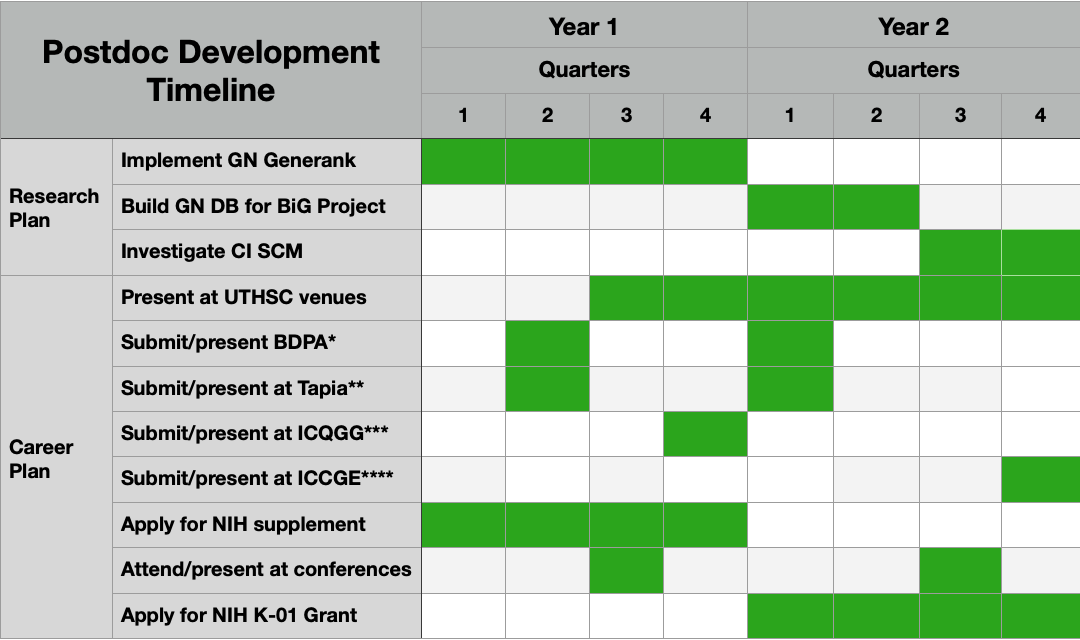
\includegraphics[width=\textwidth]{Figures/timeline-postdoc.eps}
	\caption{\textbf{Postdoc Timeline}\\
	* - Black Data Processing Associates, bdpa.org \\
	** - ACM/CMD-IT Tapia Celebration of Diversity in Computing\\
	*** - International Conference on Quantitative Genetics and Genomics\\
	**** - International Conference on Computational Genomics and Evolution
	}
	\label{fig:timeline}
\end{figure*}


%\includegraphics[width=0.4\textwidth, angle=0]{image1.pdf}